\documentclass[
BCOR0.7cm,							% Bindekorrektur, bspw. 1 cm
]
{scrbook}

\newif\ifpdf
\ifx\pdfoutput\undefined
	\pdffalse              	%normales LaTeX wird ausgef�hrt
\else
	\pdfoutput=1           
	\pdftrue               	%pdfLaTeX wird ausgef�hrt
\fi

\ifpdf %%Einbindung von Grafiken mittels \includegraphics{datei}
	\usepackage[pdftex]{graphicx} %%Grafiken in pdfLaTeX
\else
	\usepackage[dvips]{graphicx} %%Grafiken und normales LaTeX
\fi

\ifpdf
	\pdfinfo
	{
    /Author (Manfred Kindl)                                
    /Title (Tempus)     
    /Subject (Benutzerhandbuch Tempus)                                    
    /Keywords (Tempus FH-Complete Technikum-Wien)
	}
\else			
\fi

\usepackage{listings} \lstset{numbers=left, numberstyle=\tiny, numbersep=5pt}
\lstset{language=tex} 

\usepackage[pdftex,colorlinks=true,urlcolor=blue,linkcolor=blue]{hyperref}
\usepackage[ngerman]{babel}		
\usepackage[T1]{fontenc}
\usepackage[latin9]{inputenc}
\usepackage{makeidx}
\usepackage{float}
\usepackage[small,bf]{caption}
\usepackage{fancyhdr}
\usepackage{amssymb,amsmath}
\makeindex

\graphicspath{{../../images/}}

\setlength{\tolerance}{2000}
\setlength{\parindent}{0pt}
\setlength{\parskip}{1ex plus 0.5ex minus 0.2ex}
\addtolength{\textheight}{2cm}
\addtolength{\headheight}{2pt}
\setlength{\captionmargin}{20pt}
\floatstyle{plain}
\floatname{example}{Example}

\newfloat{example}{hbtp}{loe}[chapter]
\floatplacement{figure}{hbtp}
\floatplacement{table}{htbp}

\newcommand{\dollar}{\char36}

\newenvironment{info}[1]
{
    \hspace{-10mm}
    \fbox
    {
        \begin{minipage}{1cm}
        
\includegraphics[width=1cm]{icon_info}
        \end{minipage}
        \begin{minipage}{14.5cm}
        #1
        \end{minipage}
    }
}

\newenvironment{achtung}[1]{
    \hspace{-10mm}
    \fbox{
        \begin{minipage}{1cm}
        
\includegraphics[width=1cm]{icon_achtung}
        \end{minipage}
        \begin{minipage}{14.5cm}
        #1
        \end{minipage}
    }
}

\newenvironment{halt}[1]{
    \hspace{-10mm}
    \fbox{
        \begin{minipage}{1cm}
        
\includegraphics[width=1cm]{icon_halt}
        \end{minipage}
        \begin{minipage}{14.5cm}
        #1
        \end{minipage}
    }
}

\newenvironment{idee}[1]{
    \hspace{-10mm}
    \fbox{
        \begin{minipage}{1cm}
        
\includegraphics[width=1cm]{icon_idee}
        \end{minipage}
        \begin{minipage}{14.5cm}
        #1
        \end{minipage}
    }
}


\setlength{\unitlength}{1mm}

\newenvironment{markier}[5]
{    
    \thicklines \put(#2,#3){\vector(#4,#5){5}} \thinlines
    \put(#2,#3){\circle*{5}}
    \put(#2,#3){\textcolor{black}{\circle{5}}\makebox(-10,0){\textcolor{white}{#1}}}
}


\hyphenation{gleich-zeitig para-meter}


\begin{document}

\ifpdf
	\DeclareGraphicsExtensions{.pdf,.jpg,.png}
\else
	\DeclareGraphicsExtensions{.eps}
\fi

\pagestyle{fancyplain}
% Titelseite einbinden

%
% Titelseite, Abstrakt, Danksagung und Inhaltsverzeichnis
%
%% eigene Titelseitengestaltung %%%%%%%%%%%%%%%%%%%%%%%%%%%%%%%%%%%%%%%    

\begin{titlepage}
\begin{center}
\vspace*{30mm} \Huge TEMPUS\\
\vspace*{10mm}
\large \textsc{Version 2.0}

\vfill 
\includegraphics[width=136mm]{TempusLogo}\\
\vspace*{20mm}
\textsc{\LARGE{HANDBUCH}\\
\vspace*{5mm}
\large{2. Ausgabe\\Stand \today}}

	
\vfill \textsc{Technikum Wien}\\

Wien, \today
\end{center}
\end{titlepage}



\tableofcontents			% Inhaltsverzeichnis

\frontmatter					% Vorspann (z.B. r�mische Seitenzahlen)

\chapter{Einleitung}
\label{Kapitel Einleitung}


Dieses Handbuch erl�utert detailliert die Funktionen des Programms TEMPUS\raisebox{1ex}{\tiny \copyright} Version 2.0.

Das Programm wurde von Christian Paminger basierend auf XML entwickelt und programmiert.

TEMPUS\raisebox{1ex}{\tiny \copyright} ist ein Werkzeug zur Erstellung, Wartung und Modifikation von Stundenpl�nen an Hochschulen, insbesondere an Fachhochschulen und erlaubt es mehreren Usern gleichzeitig, an der selben Datenbank und dem selben Stundenplan zu arbeiten.
Die Bearbeitung erfolgt wochenweise basierend auf Kalenderwochen.
Die Steuerung geschieht haupts�chlich per Drag\&Drop.

Es ist darauf zu achten, dass derzeit noch keine vollst�ndige ''R�ckg�ngig-Funktion'' in das Programm integriert wurde. Alle �nderungen werden sofort in die Datenbank �bernommen und k�nnen nur schwer rekonstruiert werden.

TEMPUS\raisebox{1ex}{\tiny \copyright}  arbeitet mit zwei Datenbanktabellen, die sich in regelm��igen Abst�nden synchronisieren.
Gearbeitet wird in erster Linie auf der Tabelle ''Stundenplandev'' (Entwicklungsoberfl�che), die jede Nacht in die Tabelle ''Stundenplan'' kopiert wird.
Die Tabelle ''Stundenplan'' ist die Onlinetabelle, die von Studenten und Lektoren abgerufen wird.
Bis zu einem gewissen Grad erlaubt diese Absicherung ein Wiederherstellen von gel�schten Daten.
Dennoch sollte die Stundenplanung sorgf�ltig und �berlegt  durchgef�hrt werden, da eine Rekonstruktion der Daten schwierig ist. Gerade beim L�schen von Daten ist dies ratsam.
Dieser Aufbau ist dar�ber hinaus die Basis f�r die automatische Infomail, die beim Synchronisieren alle �nderungen an die betroffenen Studenten und Lektoren kommuniziert.


\begin {figure}
	\centering
	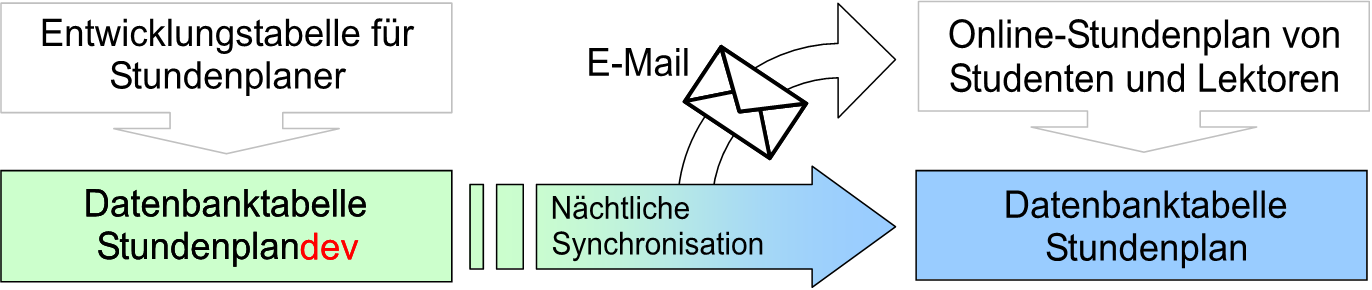
\includegraphics[width=1.0\textwidth]{SynchroSchema}
	%\caption{LE-Eigenschaften}
	\label{Schema}
\end {figure}

\achtung{�nderungen in der Onlinetabelle werden nicht in die Entwicklungsoberfl�che �bernommen. Deshalb m�ssen Sie dringende �nderungen immer in beiden Tabellen durchf�hren.
Es werden jede Nacht nur die Daten der Tabelle ''Stundenplandev'' �bernommen!}

\info{Auf Grund von unterschiedlichen Berechtigungen sind eventuell nicht alle in diesem Handbuch beschriebenen Features verf�gbar}


\mainmatter						% Hauptteil

%% Kapitel Anfang %%%%%%%%%%%%%%%%%%%%%%%%%%%%%%%%%%%%%%%%%%%%%%%%%


\chapter{Begriffserkl�rung, Features und verwendete Abk�rzungen}
\label{Kapitel Begriffe}

	\minisec{Einheit}
...siehe Lehreinheit.
	
	\minisec{Fachbereich}
...siehe Institut.

	\minisec{Institut}
Ein Institut ist die zust�ndige Stelle f�r die Vergabe von Lektoren an die einzelnen Studieng�nge und Lehrf�cher.
Ein Beispiel ist das Institut ''Sprachen'', der f�r alle sprachbezogenen Lehrf�cher zust�ndig ist. (Englisch, Franz�sisch, Japanisch,...)

	\minisec{Kollision}
TEMPUS\raisebox{1ex}{\tiny \copyright} 2.0 �berpr�ft bei Eintragungen und Verschiebungen im LV-Plan die Verf�gbarkeit von Lektoren, Studenten und R�umen, sowie Zeitsperren der Lektoren und Reservierungen. Sollte es zu einer Terminkollision mit einem der drei Pl�ne kommen, erscheint eine Fehlermeldung und die Aktion wird abgebrochen.
Durch Deaktivieren der Kollisions�berpr�fung im Men�punkt ''Einstellungen'' kann jedoch eine Kollision erzwungen werden. Dies sollte jedoch stets nach Gebrauch wieder deaktiviert werden, da es sonst leicht zu Fehlplanungen kommen kann. (siehe Kapitel \ref{Kapitel Kollisionen})

	\minisec{KW...Kalenderwoche}
Das Jahr umfasst mindestens 52 durchnummerierte Kalenderwochen (KW). Die erste Woche des Jahres nach DIN 1355 / ISO 8601 ist die erste Woche, in die mindestens vier Tage des neuen Jahres fallen. 

	\minisec{Kollegium}
Das Kollegium setzt sich aus allen StudiengangsleiterInnen sowie VertreterInnen der Lehrenden, FachbereichsleiterInnen und StudentInnen zusammen und trifft wichtige strategische Entscheidungen f�r die Fachhochschule Technikum Wien.
	
	\minisec{LE...Lehreinheit}
In der Lehreinheit verschmelzen die wesentlichen, ver�nderlichen Daten um mit der Planung fortfahren zu k�nnen. Die Daten in den Lehreinheiten dienen speziell f�r die LV-Planung und auch als Datenquelle f�r die CIS-Seite. Lehrauftr�ge werden auch auf Basis dieser Daten erstellt. 

Die Lehreinheit f�hrt Lektoren, Studenten, Lehrf�cher usw. zusammen und muss jedes Semester �berarbeitet werden.

Eine detailierte Beschreibung finden Sie in Kapitel \ref{Kapitel Lehreinheiten}

Siehe zum Vergleich ''LV...Lehrveranstaltung''

	\minisec{Lehreinheit\_ID}
Die Lehreinheit\_ID ist eine interne Nummer, die vom System eindeutig jeder Lehreinheit zugeteilt wird.
Die meisten Tabellen der Datenbank sind mit der Lehreinheit\_ID verkn�pft

	\minisec{Lehrfach}
Ein Lehrfach bestimmt den Inhalt einer Lehreinheit. (z.B. Mathematik)

In ihr definiert sind der verantwortliche Fachbereich, die Farbe (die im Stundenplan angezeigt wird) und die Unterrichtssprache. Ein Lehrfach wird f�r jeden Studiengang und jedes dazugeh�rige Semester angelegt. Die Kurzbezeichnung des Lehrfachs wird gemeinsam mit der Lehrform an erster Stelle im Lehrveranstaltungsplan angezeigt. 
Die Lehrform des Unterrichts (�bung, Vorlesung, ILV, ...) wird hier jedoch nicht bestimmt.

	\minisec{Lehrform}
Die Lehrform beschreibt das Lehrfach detaillierter, indem sie angibt, in welchem Stil der Unterricht stattfindet. 

Eine Lehrform kann Beispielsweise die Vorlesung (-VO) sein. Dies beschreibt einen Frontalunterricht ohne selbstst�ndige �bungen. 

Andere Beispiele sind �bung (-UE), Integrative Lehrveranstaltung (-ILV), Laborstunden (-LAB) oder Tutorien (-TUT)

	\minisec{Lehrveranstaltungsplan (=Stundenplan)}
Der Lehrveranstaltungsplan (kurz ''LV-Plan'') ist die Oberfl�che auf der graphisch die Lehreinheiten mit den unterrichtenden Lektoren, dem Lehrverband und dem Raum farblich dargestellt werden. 

Am LV-Plan kann durch die R�ume und die Unterrichtswochen gebl�ttert werden und der LV-Plan kann dort auch f�r diverse andere Anwendungen exportiert werden.

	\minisec{Lehrverband}
Der Lehrverband bezeichnet die Gliederung der Studenten in Studiengang, Semester, Verb�nde und Gruppen. 

Er dient der Schlichtung und Aufteilung gr��erer Studentenzahlen um kleinere und �bersichtlichere Gruppen zu schaffen. 

Ein Beispiel an der FH Technikum-Wien w�re: BEL-2A1. (Studiengang Bachelor Elektronik, 2. Semester, Verband A, Gruppe 1) 

	\minisec{LFVT...Lehrf�cherverteilung}
Die Lehrf�cherverteilung ist die gesamte Liste aller Lehreinheiten, die in einem Semester eines Studienganges zu verplanen sind.

	\minisec{LV...Lehrveranstaltung}
Als Lehrveranstaltung wird im Gesamtsystem das gleiche verstanden, wie im Antrag des Studiengangs. In ihr enthalten sind die grundlegenden Stammdaten. Im Gegensatz zu der Lehreinheit enth�lt die Lehrveranstaltung Daten, die im Wesentlichen von Jahr zu Jahr unver�ndert bleiben. Sie bildet das Grundger�st auf dem alle anderen Tabellen aufbauen.\\
Die Lehrveranstaltung wird immer aus Sicht eines Studiengangs oder aus der Sicht des Studenten gesehen. Der Titel der Lehrveranstaltung findet sich im Zeugnis und im Lehre-Bereich im CIS wieder. Nicht zu verwechseln ist die Lehrveranstaltung mit dem Lehrfach oder der Lehreinheit (siehe eigene Begriffserkl�rungen).\\
Einmal verwendete Lehrveranstaltungen k�nnen nicht mehr entfernt sondern nur deaktiviert werden, da Notenzuordnungen verloren gehen w�rden.

Attribute der Lehrveranstaltung sind beispielsweise die Kurzbezeichnung, der Studiengang, das Semester in dem diese unterrichtet wird, die Sprache, die ECTS-Punkte oder die Semesterstunden.

	\minisec{Module, Spezialgruppen}
Neben den regul�ren Lehrverbandsgruppen gibt es Module und Spezialgruppen, die unterschiedliche Studenten beherbergen k�nnen.
Es ist damit m�glich, Studenten aus verschiedenen Lehrverbandsgruppen innerhalb eines Semesters aber auch semester- und studiengangs�bergreifend zusammenzufassen. Da eine Kollisionspr�fung und korrekte Verplanung durch Spezialgruppen aber erheblich erschwert wird, sollten Spezialgruppen m�glichst vermieden werden.

	\minisec{Quickinfo}
Eine Quickinfo erscheint, wenn der Mauszeiger l�ngere Zeit ohne zu klicken �ber einem Element steht.

	\minisec{Raumtyp}
Um die verschiedenen Unterrichtsr�ume zusammenzufassen, wird das Attribut ''Raumtyp'' verwendet.
Ein Raumtyp w�re beispielsweise ''Seminarraum''. Dieser fasst beliebig viele, einzelne R�ume zu einer Gesamtheit zusammen.
Das Attribut dient haupts�chlich dazu, um bei der Stundenverplanung eine �bersichtliche Menge an Raumvorschl�gen f�r eine Lehreinheit zu erhalten.

	\minisec{Reservierung}
Der Lehrveranstaltungsplan bietet Lektoren und Angestellten die M�glichkeit der Reservierung, um sich mittelfristig einen Raum zu sichern und f�r die Lehrveranstaltungsplanung und andere Mitarbeiter zu sperren.
Die Reservierung eines Raumes ist in einem vordefinierten Zeitfenster m�glich. Eine get�tigte Reservierung hat normalerweise Vorrang vor dem regul�ren Unterricht.

Dies stellt sich in der Praxis aber als �u�erst hinderlich dar. Oft sind externe Veranstaltungen, Gastvortr�ge, Feiern und Sponsionen ein Grund f�r unangenehme Verschiebungen und Raumzuteilungen. Jene irregul�ren Veranstaltungen sind aber ein wichtiger Teil des Fachhochschulbetriebs und so wird sich vermutlich keine angenehmere L�sung finden lassen, als solchen Veranstaltungen Vorrang zu geben.

	\minisec{Semester (Jahrgang)}
Ein Semester (von lat.: sex=sechs; mensis=Monat) ist ein Studienhalbjahr an einer Hochschule. Dabei sind die Semesterferien (=vorlesungsfreie Zeit) einbezogen.
F�r gew�hnlich sind ungerade Semester (1,3,5,...) im Wintersemester (von September bis Februar) und gerade Semester (2,4,6,...) im Sommersemester (von M�rz bis August) 

	\minisec{Spezialgruppen}
...siehe Module

	\minisec{Studiengang}
Ein Studiengang ist ein, hinsichtlich eines Studienabschlusses eines wissenschaftlichen Studienfaches, angebotener Lerninhalt an einer Hochschule. 

Das Curriculum eines Studienganges wird durch die Studienordnung, die Pr�fungsleistungen und den Abschluss durch die Pr�fungsordnung definiert. 

Ein Studiengang schlie�t mit einem akademischen Grad zum Beispiel Diplom, Bachelor oder Master ab.

	\minisec{Studiensemester}
Das Studiensemester ist eine eindeutige Zuordnung zu einem Semester und einem Kalenderjahr.
Demnach ist ''WS2007'' das Wintersemester im Jahr 2007.

	\minisec{Stundenblockung}
Die Stundenblockung gibt an, wie viele Einheiten am St�ck (also direkt hintereinander) verplant werden sollen. Da (bei Einheiten zu 45 Minuten) eine Einzelstunde oft unzureichend ist, wird die Stundenblockung in den meisten F�llen zumindest ''2'' betragen.

	\minisec{Stundenplan}
...siehe Lehrveranstaltungsplan

	\minisec{UNR...Unterrichtsnummer}
Die Unterrichtnummer ist eine fortlaufende Zahl, die vom System automatisch generiert wird und haupts�chlich f�r Abl�ufe im Hintergrund relevant ist. Normalerweise wird die UNR gleichgesetzt mit der Lehreinheit\_ID. 
Wichtig zu wissen ist, dass die Kollisions�berpr�fung des LV-Plans anhand der UNR erfolgt. Lehreinheiten mit der gleichen UNR k�nnen also parallel verplant werden, ohne dass eine Fehlermeldung erfolgt.

	\minisec{Unterrichtseinheit}
Ein Tag kann in beliebig viele Unterrichtseinheiten mit einer Beginn- und Endzeit aufgeteilt werden. Dabei d�rfen sich allerdings die Beginnzeiten nicht �berschneiden.
Am Beispiel Technikum-Wien erfolgt die Unterteilung in 16 Einheiten zu je 45 Minuten, beginnend mit 08:00 Uhr.

	\minisec{Wochenrhythmus}
Wird eine Lehrveranstaltung in regelm��igen Abst�nden �ber das Semester verteilt, kann beim Attribut ''Wochenrhythmus'' das Intervall angegeben werden.
Ein Wochenrhythmus ''2'' bedeutet demnach, dass die LV alle 2 Wochen stattfinden soll.

	\minisec{Zeitsperre}
Die Zeitsperre ist eine Erweiterung des Features ''Zeitwunsch'', um detailliertere Informationen zur Verf�gbarkeit eines Lektors zu bekommen.
Der/DIe LektorIn erh�lt dadurch die M�glichkeit, unbegrenzt viele Termine punktuell zu sperren (Beispielsweise wegen Konferenzen, Auslandsaufenthalten, Urlaub oder Schulungen). Eine Zeitsperre wird im LV-Plan dunkelrot hervorgehoben und erzeugt beim verplanen eine Kollision. (siehe Kapitel \ref{Kapitel Kollisionen})

	\minisec{Zeitwunsch}
Jedem/Jeder LektorIn wird in seinem Profil die M�glichkeit gegeben, Zeitpr�ferenzen f�r seinen Unterricht anhand eines Normwochenrasters einzutragen. Der Lektor kann f�r jeden Tag und jede Unterrichtseinheit einer Woche Gewichtungen von -2 bis +2 geben um so seine Verf�gbarkeit anzugeben. Dieses Muster wird dann f�r alle Wochen eines Semesters �bernommen.
Die Zeitw�nsche sollen nach dem Fairplay-Prinzip gew�hlt werden, so dass mindestens doppelt so viele positiv bewertete Einheiten vorhanden sind, wie laut Lehrauftrag zu unterrichten w�ren.

\begin{tabular}{rll}
+2&...&hier m�chte ich unterrichten\\
+1&...&hier kann ich unterrichten\\
-1&...&hier nur in Notf�llen\\
-2&...&hier kann ich gar nicht unterrichten\\
\end{tabular}

Die Werte werden durch ein Farbsystem (von Rot bis Gr�n) im Hintergrund angezeigt. Die Standardeinstellung ist +1. 

Die Praxis zeigt aber, dass Lektoren dieses Feature oft nicht in Anspruch nehmen oder derart in der Flexibilit�t eingeschr�nkt sind, dass eine reibungsfreie Planung nicht m�glich ist. In Einzelf�llen werden sogar weniger Einheiten positiv bewertet, als pro Woche zu unterrichten sind.
Au�erdem werden die Zeitw�nsche selten auf den neuesten Stand gebracht, was wiederum zu nachtr�glichen �nderungen f�hrt.
Ein disziplinierter Gebrauch der Zeitw�nsche ist also ein wesentlicher St�tzpunkt f�r eine effektive Lehrveranstaltungsplanung.

Im Programm TEMPUS\raisebox{1ex}{\tiny \copyright} wird der Zeitwunsch bei Auswahl eines Lektors oder beim setzen einer Lehreinheit durch die Hintergrundfarbe angedeutet.

\begin{figure}
	\centering
	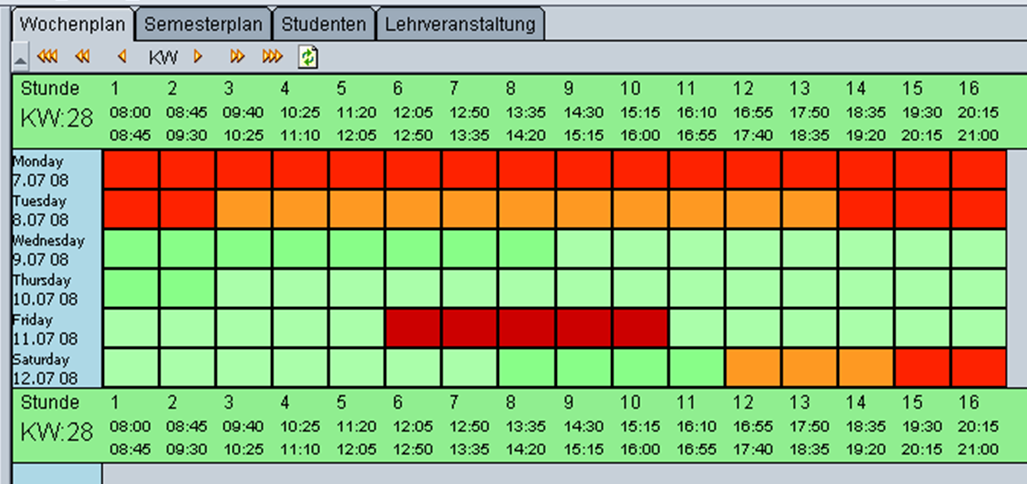
\includegraphics[width=0.8\textwidth]{Tempus_Beispiel_Zeitwunsch}
	\caption{Beispiel eines Zeitwunsches mit allen vier Werten und einer Zeitsperre (Dunkelrot) am Freitag}
	\label{Zeitwunsch}
\end{figure}
\chapter{Lehreinheiten \normalsize{(Karteireiter Lehrveranstaltung)}}
\label{Kapitel Lehreinheiten}

In der Lehreinheit verschmelzen die wesentlichen, ver�nderlichen Daten um mit der Planung fortfahren zu k�nnen. Die Daten in den Lehreinheiten dienen speziell f�r die LV-Planung und auch als Datenquelle f�r die CIS-Seite. Lehrauftr�ge werden auch auf Basis dieser Daten erstellt. 

Die Lehreinheit f�hrt Lektoren, Studenten, Lehrf�cher usw. zusammen und muss jedes Semester �berarbeitet werden.

\section{Eintr�ge vornehmen}
Ein Eintrag oder vielmehr eine �nderung der Daten hat keine direkte Auswirkung auf verplante Stunden. Wenn eine �nderung vorgenommen wird (z.B. ein neuer Lektor) muss dies der Lehrveranstaltungsplanung kommuniziert werden.

Die Bearbeitung der Lehreinheiten erfolgt in der Registerkarte ''Lehrveranstaltung''

Im Quellmen� wird wie gewohnt ein Lehrverband oder Lektor ausgew�hlt, dessen Lehreinheiten bearbeitet werden sollen.
Im Hauptfenster werden daraufhin die Lehrveranstaltungen angezeigt, die dem Verband oder Lektor zugeordnet sind.
Siehe dazu Abbildung \ref{Lehrveranstaltung}

\info{Bearbeitet werden k�nnen nur die \textit{Lehreinheiten}.
Die \textit{Lehrveranstaltungen} m�ssen schon in der Datenbank vorhanden sein, oder von einem Administrator angelegt werden.}

\begin{figure}
	\centering
	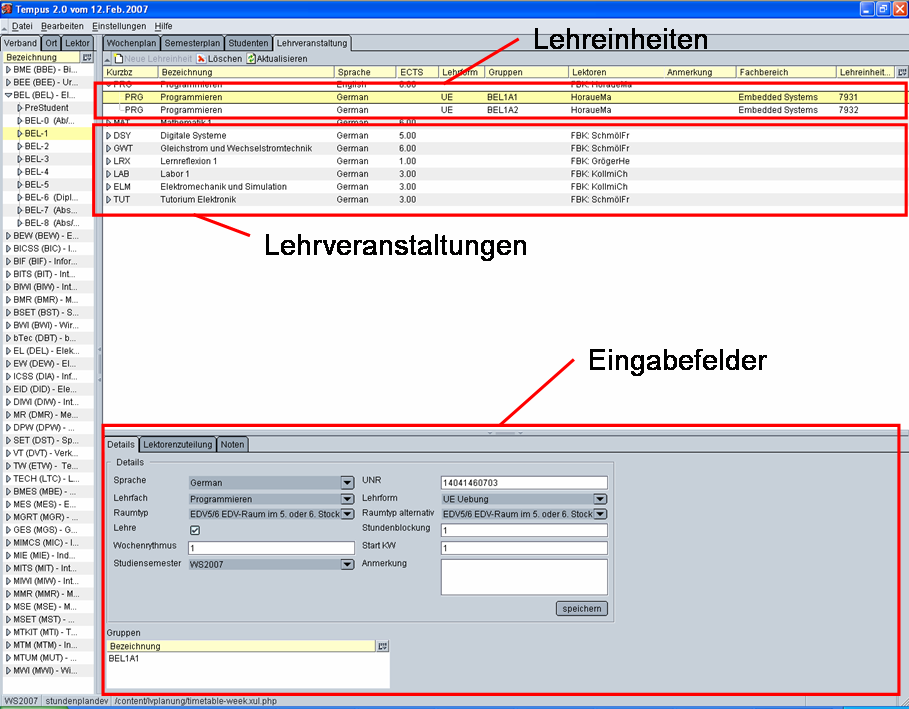
\includegraphics[width=0.8\textwidth]{Tempus_Lehrveranstaltungen1}
	\caption{Aufbau der Registerkarte \textit{Lehrveranstaltung}}
	\label{Lehrveranstaltung}
\end{figure}

Ein kleiner Pfeil neben einer Lehrveranstaltung zeigt an, dass sich darunter eine Lehreinheit befindet. Klicken Sie auf den Pfeil um die Lehreinheiten auszuklappen.

Ist noch keine Lehreinheit vorhanden (kein Pfeil), klicken Sie eine Lehrveranstaltung an. Diese wird nun \colorbox{yellow}{gelb} unterlegt. Klicken Sie nun auf\\

\includegraphics{icon_neue_LE}...neue Lehreinheit anlegen\\
um ein leeres Eingabefeld zu erhalten.
Dort k�nnen Sie nun alle Daten zu der Lehreinheit eingeben, die f�r die Verplanung notwendig sind.
In den Drop-Down Feldern, k�nnen Sie einen Eintrag aus vordefinierten Listen (wie z.B. Raumtypen) w�hlen.
% Die Bedeutung der Felder k�nnen Sie im Kapitel ''Begriffserkl�rungen'' nachschlagen.

\begin{itemize}
	\item Sprache: In welcher Sprachen wird der Unterricht abgehalten? Zur Auswahl stehen zur Zeit German, English, Espanol.
	\item UNR: Die UNR (=Unterrichtsnummer) wird nach dem Klicken auf \fbox{Speichern} automatisch generiert und ist normalerweise identisch mit der Lehreinheit\_ID. Wenn die UNR manuell mit einer anderen LE gleichgesetzt wird, findet kein Kollisionscheck im Stundenplan statt. Lehreinheiten mit gleicher UNR k�nnen demnach zeitgleich verplant werden.
	\item Lehrfach: Das Lehrfach stellt die Verbindung zum Fachbereich dar. Die Kurzbezeichnung des Lehrfachs wird gemeinsam mit der Lehrform an erster Stelle im Lehrveranstaltungsplan angezeigt. 
	\item Lehrform: Hier wird die Form des Unterrichts ausgew�hlt, z.B. Seminar, Vorlesung oder �bung.
	\item Raumtyp und Raumtyp alternativ: Um die verschiedenen Unterrichtsr�ume �bersichtlicher zu gruppieren, wird das Attribut ''Raumtyp'' verwendet.
Ein Raumtyp w�re beispielsweise ''Seminarraum''. Dieser fasst beliebig viele, einzelne R�ume zu einer Gesamtheit zusammen.
Das Attribut dient haupts�chlich dazu, um bei der Stundenverplanung eine �bersichtliche Menge an Raumvorschl�gen f�r eine Lehreinheit zu erhalten.
	\item Lehre: Wenn angehakt, wird diese Lehreinheit in den Stundenplan einbezogen.
	\item Stundenblockung: Gibt an, wie viele Einheiten am St�ck (also direkt hintereinander) verplant werden sollen. Da (bei Einheiten zu 45 Minuten) eine Einzelstunde oft unzureichend ist, wird die Stundenblockung in den meisten F�llen zumindest ''2'' betragen.
	\item Wochenrythmus: Der Wochenrythmus gibt an, in welchem Intervall (z.B. ''1'' f�r w�chentlich oder ''2'' f�r einen 14-t�gigen Rhythmus) der Unterricht stattfindet.
	\item Start KW: Die Start-Kalenderwoche gibt die Wochen an, in der die Lehreinheit beginnen soll.
	\item Studiensemester: Hier wird ausgew�hlt, in welchem Studiensemester der Unterricht stattfindet (z.B. WS2007).
	\item Anmerkung: Besonderheiten, die bei der Erstellung des Stundenplans ber�cksichtigt werden sollen, k�nnen hier eingegeben werden. 
	\end{itemize}

\section{Gruppen zuweisen}

In dem wei�en Feld ''Gruppen'' k�nnen nun die Lehrverb�nde definiert werden, die der Lehreinheit zugeordnet werden sollen.
Das Feld kann durch Drag\&Drop aus dem Quellmen� bef�llt werden. Klappen Sie den gew�nschten Verband im Quellmen� auf und ziehen Sie ihn in das Feld ''Gruppen''. Es k�nnen mehrere Gruppen zugewiesen werden.

Sie k�nnen einzelne Gruppen l�schen, indem Sie diese markieren, mit der rechten Maustaste anklicken, und \textit{Entfernen} dr�cken.

\section{Lektoren zuweisen}

Im n�chsten Schritt erfolgt die Zuweisung der Lektoren zur Lehreinheit.
Wechseln Sie dazu im Eingabefeld den Karteireiter auf ''Lektorenzuteilung'' und im Quellmen� auf die Karteikarte ''Lektor'' wie in Abbildung \ref{Lektorenzuteilung} dargestellt ist.

\begin{figure}
	\centering
	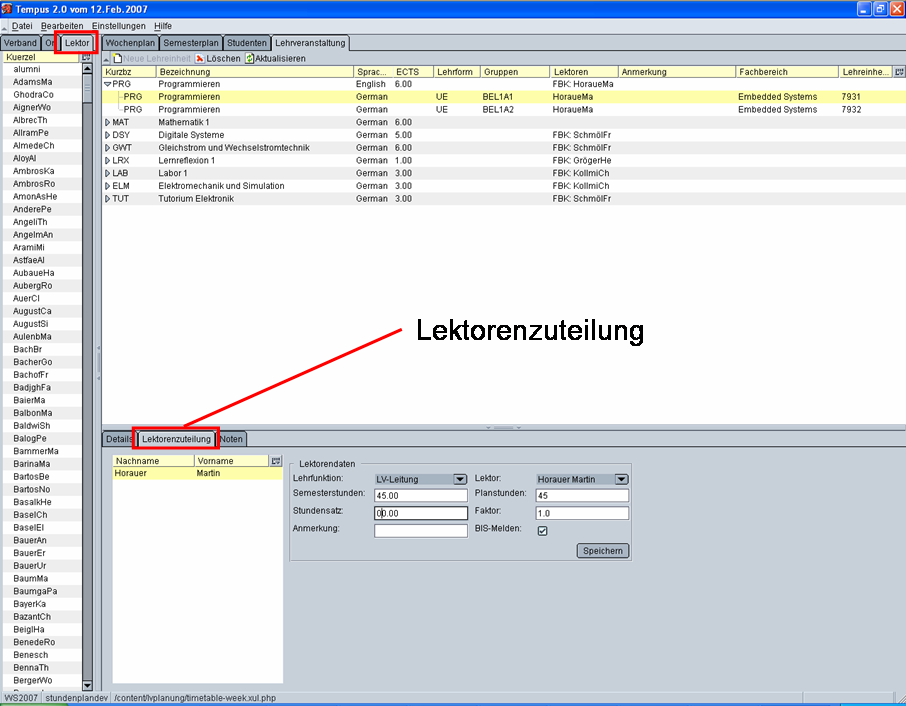
\includegraphics[width=0.8\textwidth]{Tempus_Lehrveranstaltungen2}
	\caption{Registerkarte Lektorenzuteilung}
	\label{Lektorenzuteilung}
\end{figure}

Nun k�nnen Sie per Drag\&Drop aus dem Quellmen� einen oder mehrere Lektoren in das wei�e Feld ziehen.
Wenn Sie danach einen Lektor anklicken, k�nnen Sie daneben die Lektorendaten eingeben oder �ndern.

\begin{itemize}
	\item Lehrfunktion: Hier wird die Funktion der Person innerhalb der Lehreinheit bestimmt.
	\item Lektor: Diese Feld dient dazu, den eingetragenen Lektor zu �ndern, wenn dieser schon verplant wurde. (siehe Kapitel \ref{Lektoren �ndern})
	\item Semesterstunden: Hier wird die Stundenanzahl definiert, die der Lektor tats�chlich bezahlt bekommt. Dezimalangaben sind dabei erlaubt (Trennung durch einen Punkt). Diese Zahl wird abgerundet als ganze Zahl in das Feld ''Planstunden'' �bernommen.
	\item Planstunden: Die Planstunden werden in der Lehrf�cherverteilung in TEMPUS\raisebox{1ex}{\tiny \copyright} angezeigt und sind die Stunden, die im LV-Plan verplant werden sollen.
Im Normalfall werden Semesterstunden und Planstunden �bereinstimmen.
Sollte jedoch eine Abweichung beabsichtigt sein, k�nnen die Planstunden ver�ndert werden.
	\item Stundensatz: Eine Dezimalzahl, die in \textit{Euro} angibt, wie viel der Lektor pro Einheit bezahlt bekommt.
	\item Faktor: Der Faktor wirkt sich auf den Stundensatz aus und wird bei der Berechnung des Lehrauftrages multipliziert. Standardm��ig ist der Faktor auf 1.0 gestellt. Wenn z.B. eine Mehrbelastung durch eine gro�e Studentenzahl besteht, kann mit einer Erh�hung des Faktors das Entgelt f�r diese Lehreinheit erh�ht werden.
	\item Anmerkung: Hier k�nnen zus�tzliche Informationen eingegeben werden.
	\item BIS-Melden: Eingabe, ob dieser Unterricht in der BIS-Meldung ber�cksichtigt wird. 
\end{itemize}

Durch dr�cken auf \fbox{Speichern} werden die Daten gesichert.
Wenn Sie danach in der Registerkarte ''Details'' auf \fbox{Speichern} dr�cken, aktualisiert sich die Liste der Lehrveranstaltungen.

Sie k�nnen Lektoren aus der Zuteilung l�schen, indem Sie diese markieren, mit der rechten MAustaste anklicken und \textit{Entfernen} w�hlen.
Ein Lektor kann nicht gel�scht werden, wenn er bereits im Stundenplan verplant wurde. In diesem Fall erscheint eine Fehlermeldung.

\idee{Die Liste der Lehrveranstaltungen kann durch klicken auf die �berschrift sortiert werden.}

\info{Werden pro Lehreinheit mehrere Gruppen und/oder mehrere Lektoren angegeben, gibt dies der Planungsstelle zu verstehen, dass diese Lehreinheiten auch nur so stattfinden. Zwei zugeteilte Lektoren bedeuten demnach, dass zwei Lektoren zur selben Zeit, im selben Raum, die selbe Gruppe unterrichten.}


\includegraphics{icon_aktualisieren}...Durch klicken auf das Symbol, aktualisiert sich die Liste der Lehrveranstaltungen.


\includegraphics{Listenfeld_ConfigButton}...Dieser Button blendet zus�tzliche Details in der Liste der Lehrveranstaltungen ein.

\section{Lektoren �ndern}
\label{Lektoren �ndern}

Die folgende M�glichkeit ist gerade beim �ndern von Dummy- oder NN-Lektoren hilfreich aber auch um jeden bereits verplanten Lektor durch einen anderen zu ersetzen.
Es ist nicht zwingend notwendig, den alten Lektor zu l�schen und einen neuen Lektor an den selben Terminen zu verplanen.\\

W�hlen Sie in der Registerkarte ''Lehrveranstaltung'' die betreffende Lehreinheit aus und gehen Sie dort auf die Registerkarte ''Lektorenzuteilung''. Klicken Sie den Lektor an, den Sie ersetzen m�chten. Im Drop-Down Feld w�hlen Sie nun den neuen Lektor aus und dr�cken auf  \fbox{Speichern}.\\
Wenn diese �nderung keine Kollision im LV-Plan verursacht, wird der alte Lektor gleich im LV-Plan ersetzt. Sollte aber eine Kollision entstehen (auch bei Zeitsperren) muss die Lehrveranstaltungsplanung diese erst in BEIDEN Stundenplantabellen beseitigen oder ggf. den alten Lektor l�schen und den neuen Lektor h�ndisch verplanen.

\begin{figure}
	\centering
	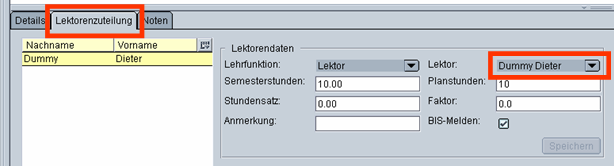
\includegraphics[width=0.8\textwidth]{Tempus_Lektor_aendern}
	\caption{Einen bereits verplanten Lektor nachtr�glich �ndern}
	\label{Lektor �ndern}
\end{figure}

\section{Eintr�ge l�schen}

Angelegte Lehreinheiten k�nnen auf 2 Arten gel�scht werden.

Entweder durch markieren der Lehreinheit und klicken auf den Button 

\includegraphics{delete}...''Lehreinheiten l�schen'' oder durch markieren, klicken mit der rechten Maustaste und dr�cken auf ''Entfernen''.

Zugeteilte Lektoren und Gruppen werden ebenfalls durch markieren und der rechten Maustaste gel�scht.

Wenn eine Lehreinheit bereits im LV-Plan verplant wurde, ist das L�schen der Lehreinheit, eines zugeteilten Lektors und einer Gruppe NICHT m�glich.

Zuvor m�ssen alle verplanten Lehreinheiten aus den Tabellen Stundenplan UND StundenplanDEV entfernt werden.
\chapter{Die Benutzeroberfl�che}
\label{Kapitel Benutzeroberfl�che}

\begin {figure}
	\centering
	\includegraphics[width=1.0\textwidth]{Tempus_Oberfl�che_Beschriftet}
	\caption{Gliederung der Benutzeroberfl�che}
	\label{Benutzeroberfl�che}
\end {figure}

\section{Hauptmen�}

\includegraphics{eins}
Im Hauptmen� k�nnen Sie die grundlegenden Einstellungen vornehmen.
Im Punkt ''Einstellungen'' w�hlen Sie das Studiensemester, das Sie bearbeiten m�chten.
Hier k�nnen Sie auch auf die Onlinetabelle (Stundenplan) wechseln, in der �nderungen sofort auf dem Studentenplan sichtbar werden.
Au�erdem k�nnen Sie hier die drei verschiedenen Kollisions�berpr�fungen aktivieren und deaktivieren. (siehe Kapitel \ref{Kapitel Kollisionen})

\info{Das aktuell eingestellte Studiensemester und die aktuell aktive Datenbanktabelle werden im Fenster ganz links unten angezeigt.}

\section{Quellmen�}

\includegraphics{zwei}
Hier k�nnen Sie zwischen dem Lehrverband, dem Ort und dem Lektor w�hlen, 
welcher im Hauptfenster (4) angezeigt werden soll.
Das Quellmen� ist als Baumstruktur aufgebaut. Durch Klicken auf die kleinen Pfeile blenden Sie eine untergeordnete Gruppe ein und k�nnen diese damit auch wieder ausblenden.
Eine ausgew�hlte Zeile wird \colorbox{yellow}{gelb} markiert, was sich auch nach Wechsel des Karteireiters nicht �ndert. Der Inhalt des Hauptfensters wird an die gew�hlte Zeile angepasst.

\info{Wenn Sie den Karteireiter im Quellmen� wechseln und wiederholt einen anderen Karteireiter aufrufen, m�ssen Sie erneut auf die gelb unterlegte Zeile klicken, um die Ansicht im Hauptfenster zu aktualisieren.}

\idee{TIPP	Sie brauchen nicht die lange Liste an Lektoren h�ndisch durchscrollen. Markieren Sie einen beliebigen Lektor und geben Sie den Namen des gesuchten Lektors auf der Tastatur ein.}


\includegraphics{Listenfeld_ConfigButton}...Dieser Button blendet zus�tzliche Details im jeweiligen Karteireiter ein.

\section{Ansicht}

\includegraphics{drei}
W�hlen Sie hier die Ansicht, die im Hauptfenster dargestellt werden soll.
Beim Start wird standardm��ig der Wochenplan aus der aktuellen Kalenderwoche angezeigt.

Die Ansicht ist an das Quellmen� gekoppelt.
Um beispielsweise den entsprechenden Studiengang in der Registerkarte ''Wochenplan'' anzeigen zu k�nnen, muss im Quellmen� ein Lehrverband ausgew�hlt werden.

Die Registerkarten der Ansicht, werden ab Kapitel \ref{Kapitel Semesterplan} n�her beschrieben.
Die Registerkarte ''Lehrveranstaltung'' wird in Kapitel \ref{Kapitel Lehreinheit} genau behandelt.

\section{Bl�ttern/Aktualisieren/Aktuelle KW}

\includegraphics{vier}
In den Kalenderwochen wird mittels der Pfeile vor- und zur�ckgebl�ttert. Die Doppelpfeile bl�ttern 4 Kalenderwochen vor bzw. zur�ck. Der Dreifach-Pfeil bl�ttert 16 Kalenderwochen (1 Semester) vor bzw. zur�ck. Der rechte Button aktualisiert den Bildschirm und dessen Inhalt.
Um auf die aktuelle KW (heute) zu springen klicken Sie auf die Abk�rzung ''KW''.

\section{Hauptfenster}
\includegraphics{f�nf}
Das Hauptfenster zeigt die ausgew�hlte Ansicht an und bietet die M�glichkeit, Stunden aus der Lehrf�cherverteilung einzuteilen bzw. vorhandene Stunden zu verschieben oder zu l�schen. Wird im Hauptfenster die Lektorenansicht ausgew�hlt, ist durch die Farben im Hintergrund (Gr�n bis Rot) der Zeitwunsch des Lektors dargestellt.
Feiertage bzw. studiengangsspezifische freie Tage und Ferien werden im Hauptfenster gelb angezeigt.
Eine blinkende Lehrveranstaltung zeigt an, dass eine Kollision/Doppelbelegung vorhanden ist.
Kommt der Cursor l�ngere Zeit auf einer verplanten Einheit zu stehen, werden im Quickinfo allf�llige Anmerkungen und das �nderungsdatum der Einheit, sowie der Benutzer, der die �nderung durchgef�hrt hat, angezeigt.

\section{Balken}

\includegraphics{sechs}
Die Breite und H�he der einzelnen Frames in der Benutzeroberfl�che kann mit den Balken beliebig verschoben werden. Durch einen einfachen Klick in der Mitte eines Balkens k�nnen diese auch aus-/eingeblendet werden.

\section{Detailansichtsfenster}

\includegraphics{sieben}
Wird im Hauptfenster einmalig auf eine Lehrveranstaltung geklickt, erscheinen im Detailfenster Informationen wie die Unterrichtsnummer oder die Langbezeichnung des Lehrfachs.


\includegraphics{Listenfeld_ConfigButton}...Dieser Button blendet zus�tzliche Spalten im Detailfenster ein.

Im Detailansichtsfenster werden die Datens�tze so detailliert aufgeschl�sselt, wie sie auch in der Datenbank vorliegen.
So wird zum Beispiel jeder teilnehmende Lektor oder jede Gruppe in einer eigenen Zeile angezeigt.

Wenn Sie ein Zeile mit Ihrer rechten Maustaste anklicken, erscheint ein Kontextmen� in dem Sie zwei Optionen haben: Bearbeiten oder Entfernen.

Durch klicken auf ''Entfernen'' wird der Datensatz gel�scht. Zuvor wird noch einmal nachgefragt.

Ein Klick auf ''Bearbeiten'' �ffnet ein Formularfeld, in dem Sie einige Parameter �ndern k�nnen. Unter anderem k�nnen Sie der Lehreinheit einen Titel geben (der im Quickinfo angezeigt wird), die UNR �ndern oder Ort und Datum adaptieren.

\achtung{Achtung: Es erfolgt dabei KEINE Kollisions�berpr�fung!}

\section{Lehreinheiten}

\includegraphics{acht}
Hier k�nnen Stunden aus der Lehrf�cherverteilung im Hauptfenster verplant werden.
Die angezeigten Lehreinheiten ergeben sich aus der Auswahl im Quellmen�.
Wird beispielsweise der gesamte Studiengang im Quellmen� ausgew�hlt, werden alle Lehrveranstaltungen aller Semester angezeigt.
Die Lehreinheiten werden zus�tzlich durch die Auswahl eines Semesters, Verbandes, einer Gruppe oder einer Spezialgruppe gefiltert.
Wird ein Lektor im Quellmen� ausgew�hlt, werden alle ihm/ihr zugeordneten Lehrveranstaltungen angezeigt. (deshalb partizipierende LV's mit mehreren Lektoren nur �ber die Verbandsansicht verplanen)

Welche Informationen in den einzelnen Lehreinheiten angezeigt werden, entnehmen Sie bitte der Abbildung \ref{LE_Details}:

\begin {figure}
	\centering
	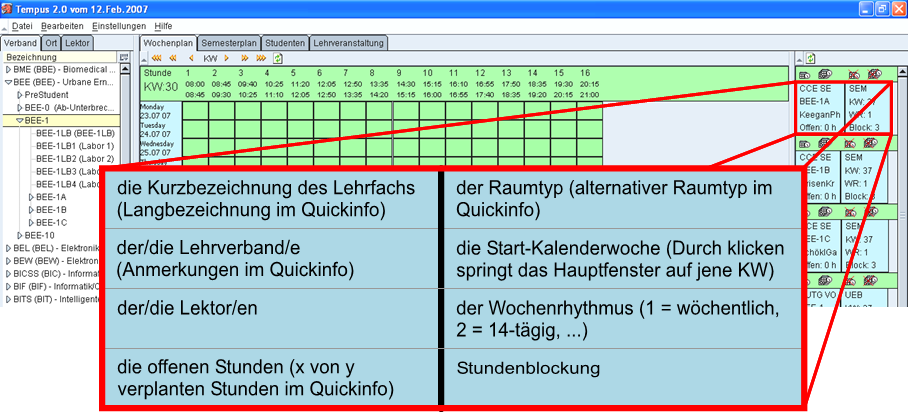
\includegraphics[width=1.0\textwidth]{Tempus_LE_Details}
	\caption{Bedeutung der angezeigten Attribute in den Lehreinheiten}
	\label{LE_Details}
\end {figure}

Die Lehreinheiten werden standardm��ig in der folgenden Hierarchie sortiert:

1. Offene Stunden\\
2. Alphabetisch nach Kurzbezeichnung der Lehreinheit\\
3. Alphabetisch nach Kurzbezeichnung der Gruppe\\
4. Alphabetisch nach Kurzbezeichnung des Lektors\\
\\
Durch die Symbole am unteren Rand kann die Sortierung ge�ndert werden.\\
\\
Um schneller die gew�nschte Lehreinheit zu finden, kann die Liste gefiltert werden. Geben sie dazu in das dar�berstehende Textfeld den gew�nschten Suchbegriff ein.\\

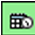
\includegraphics{single_week}...Vorschlag/Setzen SingleWeek:
Einmaliges verplanen einer Lehreinheit \textit{(in der im Hauptfenster angezeigten Kalenderwoche)}. Ein einmaliger Klick zeigt Raumvorschl�ge unter Ber�cksichtigung der Blockung und etwaiger Kollisionen im Hauptfenster an. Per Drag\&Drop kann die Lehreinheit dann in den gew�nschten Raum gezogen werden und wird dort mit der eingestellten Blockung verplant.\\
Es ist auch m�glich, ohne Raumvorschlag die Lehreinheit direkt in einen Raum zu ziehen.\\
W�hlen Sie dazu erst den Verband oder Lektor aus und wechseln Sie auf einen Raum im Quellmen�. Die angezeigten Lehreinheiten werden sich nicht ver�ndern und Sie k�nnen eine Lehreinheit direkt in einen freien Termin ziehen.
Noch einfacher ist die Verplanung �ber ein zweites Fenster, in welchem Sie einen Raum ausw�hlen und die Lehreinheit aus dem ersten Fenster per Drag\&Drop setzen. Ein Raumvorschlag ist in diesem Fall nicht notwendig.


\includegraphics{multi_week}...Vorschlag/Setzen MultiWeek:
Lehreinheit �ber das ganze Semester verplanen \textit{(beginnend bei der im Hauptfenster angezeigten Kalenderwoche)}. Ein einmaliger Klick zeigt Raumvorschl�ge unter Ber�cksichtigung der Blockung und etwaiger Kollisionen (�ber das ganze restliche Semester gesehen) im Hauptfenster an. Per Drag\&Drop kann die Lehreinheit dann in den gew�nschten Raum gezogen werden und wird dann mit der eingestellten Blockung im vorgegebenen Wochenrhythmus verplant. Dabei werden (vorher definierte) Feiertage und Ferien ausgelassen.\\
Neben dem Raumvorschlag wird in Klammer die Anzahl der Kollisionen angezeigt die durch die Verplanung entstehen w�rde. 
�ber den Men�punkt Einstellungen->max\_kollision kann festgelegt werden, wie viele kollisionen maximal vorkommen d�rfen damit der Raum vorgeschlagen wird.

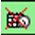
\includegraphics{delete_single_week}...L�schen SingleWeek:
Einmaliges entfernen einer Lehreinheit \textit{(aus der im Hauptfenster angezeigten Kalenderwoche)}. Dieser Button l�scht alle betreffenden Lehreinheiten aus der aktuellen Woche aus dem Plan. Davor wird allerdings noch in einem Dialogfeld nachgefragt.

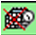
\includegraphics{delete_multi_week}...L�schen MultiWeek:
Entfernen aller verplanten Lehreinheiten \textit{(beginnend bei der im Hauptfenster angezeigten Kalenderwoche bis zum Ende des Semesters)}.
Dieser Button l�scht alle betreffenden Lehreinheiten �ber das ganze restliche Semester aus dem LV-Plan. Davor wird allerdings noch in einem Dialogfeld nachgefragt.


\includegraphics{icon_aktualisieren}...Aktualisiert die angezeigten Lehreinheiten bzw. l�dt die Ansicht neu. Damit kann auch (nach dem Raumvorschlag) die Aktion Vorschlag/Setzen Single/MultiWeek abgebrochen werden.

\section{Statusleiste}

\includegraphics{neun}
In der Statusleiste werden das aktuelle Studiensemester, die Tabelle an der gerade gearbeitet wird, sowie aktuelle Meldungen ausgegeben.

Um das Wechseln zwischen den Semestern zu erleichtern, finden Sie links in der Statusleiste 3 Buttons um das Studiensemester umzuschalten.
Die zwei Pfeile links und rechts, bl�ttern jeweils ein Studiensemester vor bzw. zur�ck.

In der Mitte steht das aktuelle Semester.
Sollten zwei oder mehr Tempus\raisebox{1ex}{\tiny \copyright}-Fenster ge�ffnet sein, erwirkt dieser Button, dass das Fenster - mit dem aktuell eingestellten Studiensemester - neu geladen wird.
\chapter{Die Stundenverplanung im Detail}
\label{Kapitel Stundenverplanung}

Hier werden detailliert die M�glichkeiten beschrieben, Stunden zu verplanen und zu l�schen.

\section{Verplanen �ber Studiengang oder Lektor}

Im Folgenden wird erkl�rt, wie die einmalige Verplanung einer LV vor sich geht.

Im Hauptfenster die gew�nschte Kalenderwoche ausw�hlen.
Den betreffenden Studiengang (ggf. auch Semester, Verband und Gruppe) oder den Lektor ausw�hlen.\\
Den ''Vorschlag/Setzen SingleWeek''-Button der gew�nschten Lehrveranstaltung dr�cken \begin{math}\rightarrow \end{math} Im Hauptfenster erscheinen nun m�gliche R�ume und im Hintergrund wird durch die Farben der Zeitwunsch des Lektors und eventuelle Zeitsperren angedeutet. Nehmen mehrere Lektoren an einer Lehreinheit teil, wird der Zeitwunsch der Lektoren auf die gemeinsame Verf�gbarkeit berechnet.\\

Dr�cken Sie nun abermals auf den Button, halten Sie die Maustaste gedr�ckt und ziehen Sie die Lehrveranstaltung an dem gew�nschten Termin in einen der vorgeschlagenen R�ume.

Das Verplanen einer durchgehenden LV �ber das ganze Semester erfolgt auf die selbe Art und Weise mit dem Unterschied, dass der ''Vorschlag/Setzen MultiWeek''-Button verwendet wird.
Dies bewirkt eine Verplanung �ber das ganze restliche Semester, beginnend ab der im Hauptfenster angezeigten KW, unter Ber�cksichtigung der eingestellten Blockung und des vorgegebenen Wochenrhythmus. Feiertage, Ferienzeiten und eventuelle Zeitsperren des Lektors werden ausgelassen.

\achtung{\underline{Bei mehreren zugeteilten Lektoren pro Lehreinheit:}\\
Achten Sie darauf, dass Sie aus der Lektorenansicht NUR den gew�hlten Lektor verplanen k�nnen. Wenn mehrere Lektoren an einer Lehreinheit teilnehmen und dies auch so verplant werden soll, muss dies aus der Lehrverbandsansicht geschehen.}

\section{Verplanen �ber Ort}
\label{Punkt Verplanen �ber Ort}

Die Lehrf�cherverteilung bietet die M�glichkeit zwei Raumtypen (Standard und Alternativ) anzugeben. Sollte nun ein anderer Raum ben�tigt werden, muss dies nicht extra in der LFVT ge�ndert werden.
W�hlen Sie wie bisher die gew�nschte Kalenderwoche und den gew�nschten Verband oder Lektor aus.
Es werden rechts die jeweiligen Lehreinheiten angezeigt.
W�hlen Sie nun im Men�fenster einen Ort \begin{math}\rightarrow \end{math} Die Liste der Lehreinheiten �ndert sich nicht.
Ziehen Sie nun ohne den Raumvorschlag zu aktivieren, den "Vorschlag/Setzen SingleWeek"-Button direkt auf den gew�nschten Termin.

\section{Verplanen �ber 2 Fenster}

Eine alternative zu der im Punkt \ref{Punkt Verplanen �ber Ort} erl�uterten Variante ist das Verplanen �ber 2 ge�ffnete Tempus-Fenster. (Sie k�nnen beliebig viele Fenster parallel �ffnen)
W�hlen Sie in einem Fenster beispielsweise einen Lektor und im zweiten Fenster einen Raum.
Sie k�nnen nun direkt, ohne einen Raumvorschlag einholen zu m�ssen, eine Lehreinheit des Lektors in einen Raum ziehen. (Bei Single- und MultiWeek m�glich).

\section{L�schen einzelner Lehrveranstaltungen}
Neben den ''L�schen SingleWeek/L�schen MultiWeek''-Buttons gibt es die M�glichkeit, einzelne Lehrveranstaltungen direkt aus dem Hauptfenster heraus zu l�schen.
Klicken Sie dazu die LV mit der rechten Maustaste an und w�hlen Sie ''entfernen''.
Best�tigen Sie mit \fbox{OK}. \\
Um mehrere Stunden auf einmal zu l�schen markieren Sie die Eintr�ge und dr�cken die Taste \fbox{ENTF}.
\label{Markieren von Stunden}
\section{Markieren von Stunden}
Sie k�nnen mehrere Stunden markieren um diese dann zu verschieben oder zu l�schen. Zum Markieren einer Stunde klicken sie mit der linken Maustaste auf eine Stunde. Um zus�tzliche Stunden zur Markierung hinzuzuf�gen, dr�cken Sie die Taste \fbox{STRG} und klicken auf die zu markierende Stunde. Diese wird dann zur Markierung hinzugef�gt.\\
Wenn Sie mehrere nebeneinander liegende Stunden markieren m�chten, markieren Sie die erste Stunde mit einem Linksklick. Dr�cken und halten Sie danach die Taste \fbox{SHIFT} und klicken auf die letzte Stunde.\\
\\
Mit einem Doppelklick auf eine Stunde werden automatisch alle zugeh�rigen Stunden (alle mit der selben UNR) an diesem Tag markiert.
\chapter{�ndern von bereits verplanten Stunden}

Ist es notwendig, eine �nderung von bereits verplanten Stunden vorzunehmen, m�ssen diese nicht unbedingt gel�scht und neu verplant werden.
Eine einfache �nderung wie beispielsweise einen Raumtausch oder eine Stundenverschiebung innerhalb der angezeigten Woche ist durch markieren und verschieben per Drag\&Drop leicht durchzuf�hren.

\section{�nderungen im selben Fenster}

Grunds�tzlich gen�gt es, eine Lehrveranstaltung direkt mit der Maus anzuklicken, die Maustaste gedr�ckt zu halten und die Lehrveranstaltung an ihren neuen Platz zu schieben. Dies setzt allerdings voraus, dass am neuen Termin der selbe Raum frei ist und auch der Lektor und die Studenten eine Terminl�cke haben. Sollte es zu einer Kollision kommen, erscheint (bei aktivierter Kollisions�berpr�fung) ohnehin eine Fehlermeldung.

\section{Verschieben nach Raumvorschlag}

Gew�hnlich ist es notwendig, bei einer Verschiebung den Raum zu wechseln.
Klicken Sie dazu mit der rechten Maustaste und dann auf Raumvorschlag auf die erste Lehreinheit der gew�nschten Lehrveranstaltung.
Im Fenster erscheinen alle freien R�ume, an allen m�glichen Terminen, unter Ber�cksichtigung aller beteiligten Lektoren und Studenten. Markieren Sie die Stunden die Sie verschieben m�chten und ziehen Sie diese auf den gew�nschten Raum.
Informationen zum Markieren finden Sie im Kapitel \ref{Markieren von Stunden}

\section{�nderungen �ber 2 Fenster}

Wird es notwendig, eine Lehrveranstaltung in eine andere Woche zu verschieben, muss dies �ber ein zweites Fenster geschehen. Verkleinern Sie dazu das ge�ffnete Fenster und �ffnen Sie TEMPUS\raisebox{1ex}{\tiny \copyright} erneut.
Ordnen Sie die Fenster unter- oder nebeneinander an, so dass Sie bequem �ber beide Fenster arbeiten k�nnen.
 
Bl�ttern Sie in einem Fenster zu der Lehrveranstaltung, die Sie verschieben m�chten. Bl�ttern Sie im 2. Fenster zu dem neuen Wunschtermin. Welche Fensterkombinationen Ihnen dabei zur Verf�gung stehen, entnehmen Sie bitte folgender Darstellung.

%\small
\begin{center}
\begin{tabular}{rcll}
AUS&&IN&FOLGE\\
\cline{1-4}
Verband&\begin{math}\rightarrow \end{math}& Raum&Raum�nderung der LV\\
Verband&\begin{math}\rightarrow \end{math}& (selber) Verband&Termin�nderung der LV\\
Verband&\begin{math}\rightarrow \end{math}& (selber) Lektor&Termin�nderung der LV\\
Lektor&\begin{math}\rightarrow \end{math}& Raum&Raum�nderung der LV\\
Lektor&\begin{math}\rightarrow \end{math}& Verband&Termin�nderung der LV\\
Raum&\begin{math}\rightarrow \end{math}& Raum&Raum�nderung der LV\\
Raum&\begin{math}\rightarrow \end{math}& Verband&Termin�nderung der LV\\
Raum&\begin{math}\rightarrow \end{math}& (selber) Lektor&Termin�nderung der LV\\
\end{tabular}
\end{center}
%\normalsize

\achtung{Achten Sie beim arbeiten mit 2 Fenstern darauf, dass in beiden Fenstern die richtige Kalenderwoche angezeigt wird. Wenn Sie in einem Fenster die Kalenderwoche �ndern, hat dies keine Auswirkungen auf die anderen ge�ffneten Fenster.}

\info{�ber 2 Fenster k�nnen die Lehrveranstaltungen nur einzeln verschoben werden. Das Markieren und Verschieben mehrerer LV ist nur im selben Fenster m�glich.}

Klicken Sie auf die Lehrveranstaltung, die Sie verschieben m�chten, halten Sie die Maustaste gedr�ckt.
Ziehen Sie die Lehrveranstaltung in das 2. Fenster an den gew�nschten Termin.
Lassen Sie die Maustaste los.
Klicken Sie im ersten Fenster auf den Button ''Aktualisieren'' 
\includegraphics{icon_aktualisieren}

\chapter{Kollisionen}
\label{Kapitel Kollisionen}

TEMPUS\raisebox{1ex}{\tiny \copyright} 2.0 �berpr�ft bei Eintragungen und Verschiebungen im LV-Plan die Verf�gbarkeit von Lektoren, Studenten und R�umen, sowie Zeitsperren der Lektoren und Reservierungen. Sollte es zu einer Terminkollision mit einem der drei Pl�ne kommen, erscheint eine Fehlermeldung und die Aktion wird abgebrochen.
Durch Deaktivieren der Kollisions�berpr�fungen kann dies umgangen werden.\\
Im folgenden werden die M�glichkeiten beschrieben, wie dies m�glich ist.

\info{Dieses Feature ist m�glicherweise wegen eingeschr�nkter Berechtigungen nicht verf�gbar}
\info{In TEMPUS\raisebox{1ex}{\tiny \copyright} wird eine Kollision durch einen blinkenden Eintrag angezeigt.}

\section{Die Arten der Kollsionen}

Im wesentlichen wird zwischen 3 Kollisionsarten unterschieden:

\begin{itemize}
\item Kollision mit eingetragenen Terminen des Lektors, der Studenten oder des Raumes
\item Kollision mit einer Reservierung
\item Kollision mit einer Zeitsperre
\end{itemize}

\section{Kollisionen erzwingen}

Sie haben im Quellmen� bei den Einstellungen die M�glichkeit, diese drei verschiedene Kollisions�berpr�fungen zu deaktivieren, bzw. zu aktivieren.

Nach anklicken einer Option signalisiert ein H�kchen, ob die �berpr�fung aktiv ist, oder nicht. Au�erdem stoppt das Blinken der kollidierenden Eintragungen im LV-Plan.\\
Eine aktivierte ''ignore\_kollision'' deaktiviert jedoch nur einen Teil der �berpr�fung. Es ist danach NICHT m�glich, eine bereits verplante Einheit, auf einen kollidierenden Termin zu schieben.
Jedoch k�nnen Sie eine Lehreinheit ohne Kollision aus der LFVT in den Plan ziehen und so eine Doppelbelegung erzwingen.\\

\achtung{SEIN SIE BEIM PLANEN OHNE KOLLISIONS�BERPR�FUNG VORSICHTIG UND AKTIVIEREN SIE DIESE WIEDER NACH GEBRAUCH.
SIE VERMEIDEN DAMIT FEHLER UND UNBEABSICHTIGTE FEHLPLANUNGEN.}\\

Eine zweite M�glichkeit eine Kollision zu erzwingen ist �ber das Detailfeld.
Klicken Sie eine Lehreinheit an. Im Detailfenster wird die Einheit nun genau aufgeschl�sselt.
Durch das Anklicken mit der rechten Maustaste k�nnen Sie nun einzelne Eintr�ge im Kontextmen� durch Ausw�hlen von ''Bearbeiten'' editieren.
Im erscheinenden Formularfeld k�nnen Sie nun \textbf{OHNE KOLLISIONS�BERPR�FUNG} verschiedene Attribute wie den Ort und das Datum der LV ver�ndern.
Dr�cken Sie anschlie�end auf \fbox{Speichern}

\section{Kollisionen auf Studentenebene}
Die normale Kollisionspr�fung pr�ft die Kollisionen anhand der Gruppen. Bei der Verwendung von mehreren Spezial- oder Modulgruppen ist dies nicht immer optimal.
Unter dem Men� Einstellungen kann die Option kollision\_student aktiviert werden. Wenn diese Einstellung aktiv ist, dann werden die Kollisionen nicht anhand der Gruppen gepr�ft sondern pro Student.\\
Bitte beachten Sie, dass diese Art der Kollisionspr�fung erst dann sinnvoll ist, wenn bereits Studenten zu den Gruppen zugeordnet wurden.\\
\\
\achtung{Diese Art der Kollisionspr�fung ist sehr Rechenintensiv und f�hrt zu l�ngeren Wartezeiten beim Verplanen.}\\

Alternativ dazu k�nnen Sie die Kollisionspr�fung auf Studentenebene auch nach der Erstellung des Planes pr�fen. Dies geschieht �ber den Men�punkt Extras->Kollision Student.

\chapter{Semesterplan}
\label{Kapitel Semesterplan}

Um eine bessere �bersicht �ber das gesamte Semester zu bekommen, kann der Semesterplan geladen werden.
Er dient nicht dazu, Stunden zu verplanen oder zu verschieben, sondern er soll den �berblick erleichtern.
Sobald Sie im Quellmen� einen Lehrverband, Lektor oder Ort ausw�hlen, wird nach wenigen Sekunden der Semesterplan generiert, in dem nun die einzelnen Wochen untereinander abgebildet werden.

\begin {figure}
	\centering
	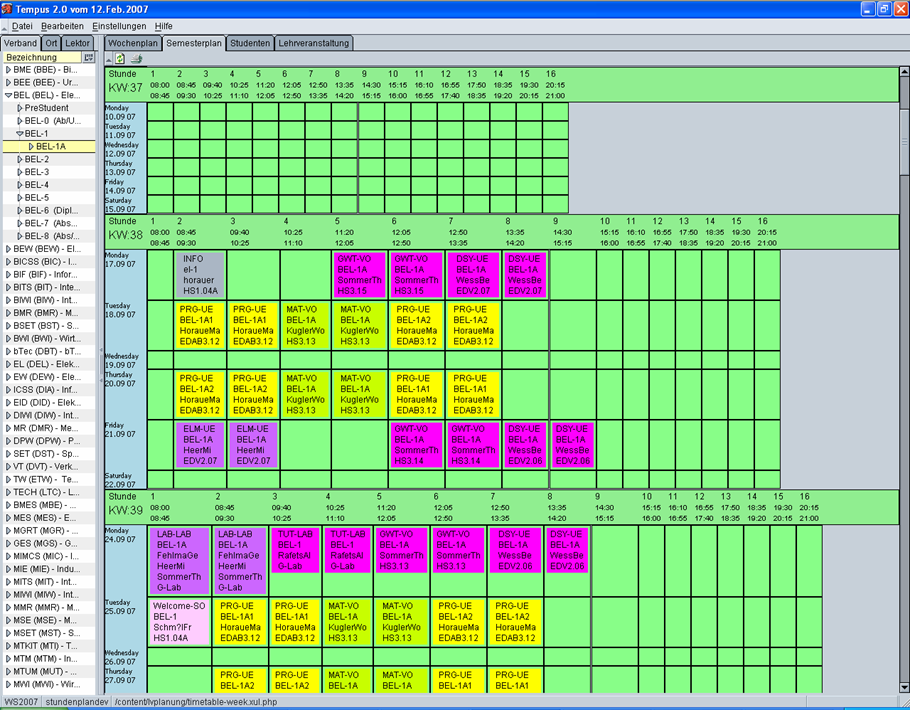
\includegraphics[width=0.8\textwidth]{Tempus_Semesterplan}
	\caption{Karteireiter Semesterplan}
	\label{Semesterplan}
\end {figure}

Wenn Sie im Quellmen� einen anderen Eintrag ausw�hlen, wird der Semesterplan angepasst.
Bei einem Wechsel der Registerkarte bleibt der Semesterplan jedoch unver�ndert erhalten.


\includegraphics{icon_aktualisieren}...Dieser Button aktualisiert den Semesterplan auf den aktuellen Stand.


\includegraphics{icon_drucken}...Ein Klick auf dieses Symbol l�dt den Semesterplan in ein Browser-Fenster von wo aus er gespeichert und gedruckt werden kann.
\chapter{Studenten}
\label{Kapitel Studenten}
Diese Registerkarte dient lediglich dazu, um der Planungsstelle einen �berblick �ber die Anzahl der Studenten in einer Gruppe zu erm�glichen.

Wenn Sie die Registerkarte ausw�hlen und im Quellmen� einen Verband oder eine Gruppe anklicken, werden die zugeordneten Studenten dieser Gruppe aufgelistet.
Au�erdem wird rechts oben, die Summe der Studenten angezeigt.


\begin {figure}
	\centering
	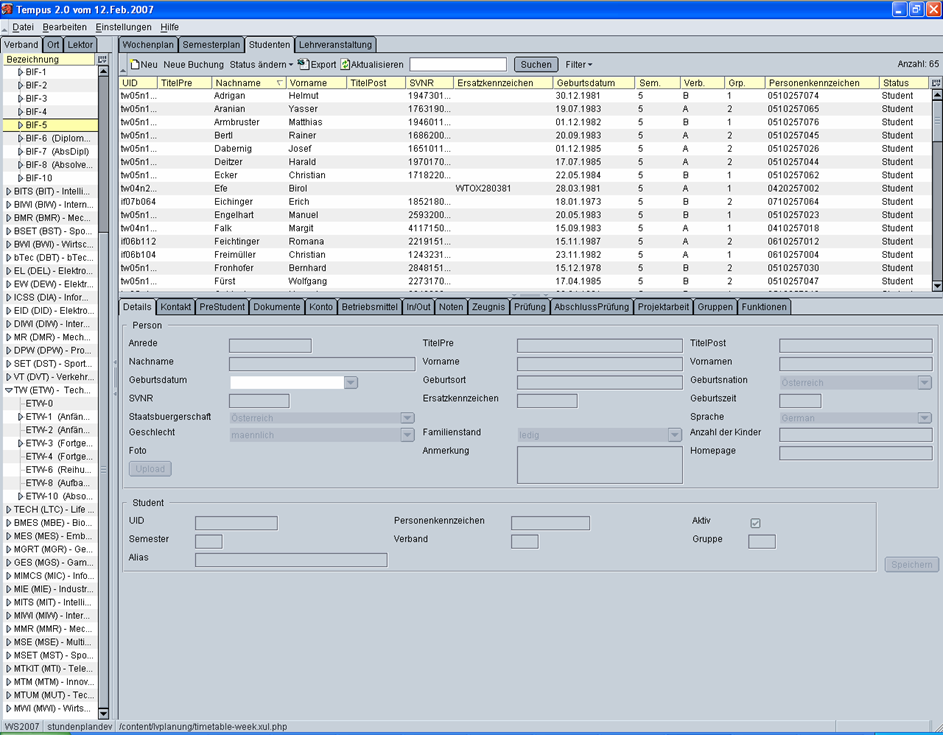
\includegraphics[width=1.0\textwidth]{Tempus_Studenten}
	\caption{Die Registerkarte ''Studenten''}
	\label{Studenten}
\end {figure}
%\chapter{Lehrveranstaltung}
\label{Kapitel Lehrveranstaltung}

Als Lehrveranstaltung wird im Gesamtsystem das gleiche verstanden, wie im Antrag des Studiengangs. In ihr enthalten sind die grundlegenden Stammdaten. Im Gegensatz zu der Lehreinheit enth�lt die Lehrveranstaltung Daten, die im Wesentlichen von Jahr zu Jahr unver�ndert bleiben. Sie bildet das Grundger�st auf dem alle anderen Tabellen aufbauen.\\
Die Lehrveranstaltung wird immer aus Sicht eines Studiengangs oder aus der Sicht des Studenten gesehen. Der Titel der Lehrveranstaltung findet sich im Zeugnis und im Lehre-Bereich im CIS wieder. Nicht zu verwechseln ist die Lehrveranstaltung mit dem Lehrfach oder der Lehreinheit (siehe eigene Begriffserkl�rungen).\\

Einmal verwendete Lehrveranstaltungen k�nnen nicht mehr entfernt sondern nur deaktiviert werden, da Notenzuordnungen verloren gehen w�rden.

Folgende Attribute bestimmen eine Lehrveranstaltung:
\begin{table*}[htbp]
	\centering
		\begin{tabular}{|r|l|}
			\hline
			Kuerzel & Abk�rzung der LV. Mindestens 2, maximal 5 Zeichen. \\&3,4 od. 5tes Zeichen darf eine Ziffer sein.\\& Buchstaben sollten einheitlich gro� geschrieben werden.\\
			\hline
			Bezeichnung & Name der Lehrveranstaltung (max. 64 Zeichen)\\
			\hline
			LehreVz	& Der Name des Lehreverzeichnisses sollte mit dem K�rzel �bereinstimmen. \\&Es sind ausschlie�lich kleingeschriebene Buchstaben zu verwenden.\\
			\hline
		\end{tabular}
	\caption{Attribute der Lehrveranstaltung}
	\label{tab:AttributeDerLehrveranstaltung}
\end{table*}

Die Registerkarte ''Lehrveranstaltung'' ist ein Grenzbereich, in dem sich die administrative Seite und die Planungsseite �berschneiden.

In der Registerkarte werden alle Daten eingegeben, die zum Verplanen im LV-Plan notwendig und relevant sind.


\section{Bearbeiten von LV-Eintr�gen}
Kommt es zu Curriculums�nderungen, stehen dem FAS-Anwender einige Anpassungsm�glichkeiten zur Verf�gung. Der Aufruf erfolgt durch Anklicken von Men�punkt \textit{Lehrveranstaltungsverwaltung} unter \textsl{Extras} wie Abbildung \ref{LV} zeigt.
\begin{figure}
	\centering
	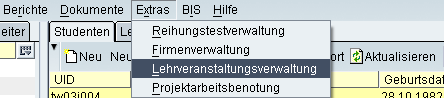
\includegraphics[width=0.75\textwidth]{FAS_LV.png}
	\caption{Bearbeiten von Lehrveranstaltungseintr�gen}
	\label{LV}
\end{figure}
Der Anwender gelangt daraufhin auf die in Abbildung \ref{LV1} gezeigte Seite in einem neuen Fenster. Zuerst werden in den Auswahlfeldern links oben, Studiengang und Semester ausgew�hlt. Zus�tzlich kann die Ausgabe auch noch auf einen Fachbereich eingeschr�nkt werden. Zum Aktualisieren der Anzeige wird dann noch die Taste \textit{Anzeigen} angeklickt. Es werden alle \underline{aktiven} Lehrveranstaltungen, die den angegebenen Kriterien entsprechen, angezeigt. Es k�nnen folgende Werte ver�ndert werden:
\begin{enumerate}
	\item Lehre: Wenn angehakt, erscheint die LV auf der CIS-Seite.
	\item Sort: Die eingegebenen Zahlen bestimmen die Reihenfolge der LVs auf dem Semesterzeugnis.
	\item Zeugnis: Wenn angehakt, erscheint die LV auf den Zeugnisausdrucken und Studienerfolgsbest�tigungen.
	\item BA/DA: Wenn angehakt, k�nnen Projektarbeiten zugeordnet werden.
	\item FBK: Hier kann ein Koordinator f�r diese LV ausgew�hlt werden. Dieses Feld mu� nur bef�llt werden, wenn der verantwortliche Koordinator nicht mit dem Fachbereichskoordinator �bereinstimmt. Bleibt das Feld leer, wird der Fachbereichskoordinator zugeordnet.
\end{enumerate}
Bei den Feldern Lehre, Zeugnis und BA/DA ist nur ein einfacher Klick und kein Doppelklick zur Zustands�nderung notwendig. Die Eingabe wird mit einem Klick auf die Taste \fbox{ok} am rechten Zeilenrand gespeichert. Mit dem Schlie�en des Fensters wird die Bearbeitung der Lehrveranstaltungen beendet.
\begin{figure}
	\begin{center}
    \begin{picture}(108,90)
			\put(0,0){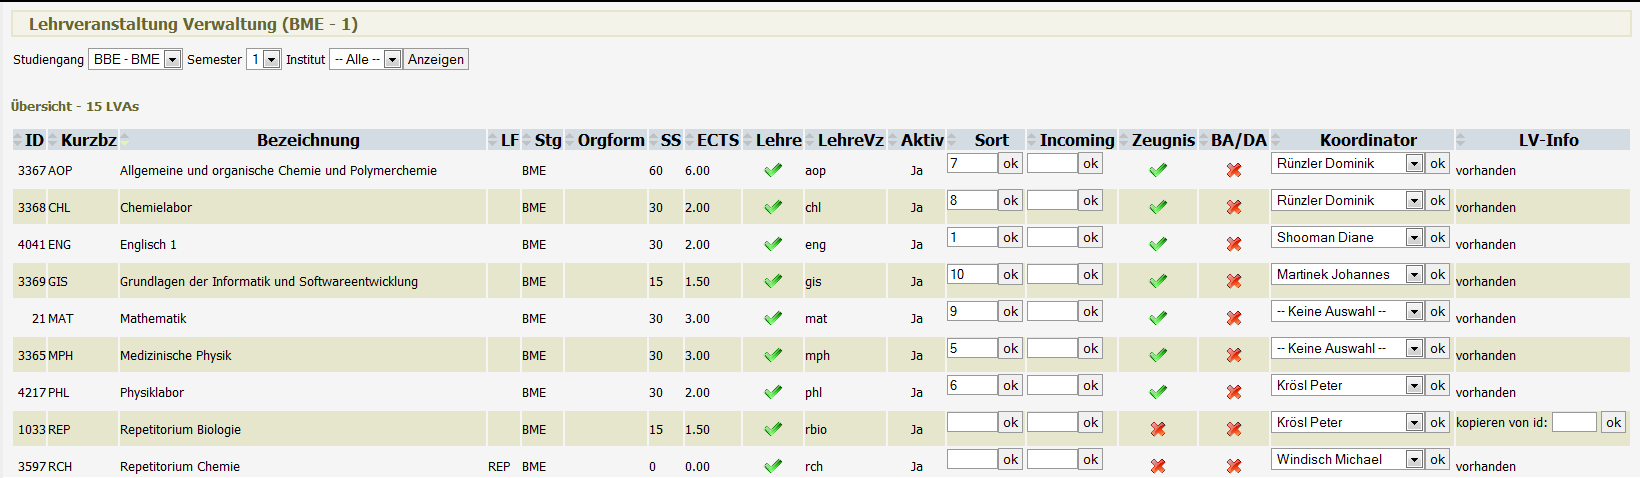
\includegraphics[height=90mm, width=108mm]{FAS_LV1.png}}
			\markier{1}{47}{81}{1}{-1}
			\markier{2}{65}{81}{1}{-1}
			\markier{3}{74}{81}{1}{-1}
			\markier{4}{82}{81}{1}{-1}
			\markier{5}{88}{81}{1}{-1}
		\end{picture}
    \caption{Lehrveranstaltungen}
		\label{LV1}
  \end{center}
\end{figure}

\chapter{Men�punkt Extras}
\label{Kapitel Extras}

Im Men�punkt ''Extras'' haben Sie diverse Zusatzm�glichkeiten, um die Planung zu erg�nzen und zu �berpr�fen.

\section{Kollision Student}

Dieser Link leitet Sie zu einer Website, auf der Sie Kollisions�berpr�fungen im Stundenplan auf Studentenebene durchf�hren k�nnen. (siehe Abbildung \ref{Kollision_Student})
Sinnvollerweise funktioniert dies erst nach erfolgter Stundenplanung und Zuteilung aller Studenten zu einer Gruppe oder Spezialgruppe.

\begin {figure}
	\centering
	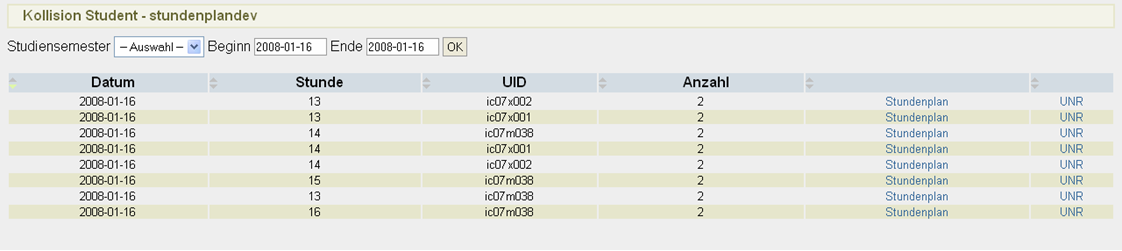
\includegraphics[width=1.0\textwidth]{Tempus_Kollisionscheck_Studenten}
	\caption{Kollisionscheck auf Studentenebene}
	\label{Kollision_Student}
\end {figure}

W�hlen Sie aus den Drop-Down Feldern das gew�nschte Studiensemester und den Zeitraum, zwischen dem �berpr�ft werden soll. Sind Beginn- und Endedatum gleich wird nur jener Tag �berpr�ft.
Wir empfehlen den Zeitraum m�glichst klein zu w�hlen, um die Berechnungszeit zu verk�rzen.

Die daraufhin generierte Liste, wird auf maximal 30 Eintr�ge beschr�nkt.
Sie k�nnen die Liste durch klicken auf die Spalten�berschriften sortieren.

In jeder Zeile finden Sie die Links ''Stundenplan'' und ''UNR'', die jeweils in der unteren Fensterh�lfte Zusatzdetails aufrufen:

Der Link ''Stundenplan'' blendet alle Stunden an diesem Tag in dieser Unterrichtseinheit ein. Mit dem Button ''Delete'' k�nnen Sie danach Eintr�ge l�schen.

Der Link ''UNR'' blendet die Studentenkollision auf Gruppenebene ein.


\chapter{Tipps und Tricks}
\label{Kapitel Tipps}

\section{Planungsablauf}

Es empfiehlt sich, die Planung der Lehreinheiten mit den Vorlesungen zu beginnen, die alle Studenten gemeinsam besuchen. Das nachtr�gliche Einpflegen solcher Stunden ist schwieriger, als L�cken f�r Teilgruppen zu finden.

\section{Falsche Stundenblockung}

Angenommen, Sie wollen eine LV �ber 3 Lehreinheiten verplanen, es ist jedoch nur eine 2-Stunden Blockung eingestellt. Es ist dann nicht unbedingt notwendig, die Blockung zu ver�ndern. Verplanen Sie zun�chst 2 LE, l�schen Sie nur die zweite (rechte Maustaste ''Entfernen''), verplanen Sie erneut 2 LE direkt danach.

\section{R�ume umschlichten}

Angenommen, Sie wollen (z.B. bei Umschlichtungen in den R�umen) zwei Lehrveranstaltungen am selben Termin in den jeweils anderen Raum schieben. Da Ihnen kein Zwischenspeicher zur Verf�gung steht und eine solche Verschiebung eine Kollision verursacht, m�ssen Sie sich mit einem Trick behelfen. Verschieben Sie zun�chst die erste LV in das zweite Fenster aber an einen Termin, der aller Wahrscheinlichkeit nach frei ist (z.B. Samstag Abend). Verschieben Sie dann die zweite LV an den freigewordenen Termin. Korrigieren Sie zuletzt die erste LV an Ihren eigentlichen Platz.

\section{Kollisions�berpr�fung �berbr�cken}

Wenn Sie in der Registerkarte ''Lehrveranstaltung'' bei einer Lehreinheit die UNR manuell gleich mit einer anderen Lehreinheit setzen, kollidieren diese bei der Verplanung nicht.
%\chapter{Installation von Tempus}
\label{Installation}

Tempus ben�tigt einen XUL-Unterst�tzenden Browser im Hintergrund.

Es wird empfohlen, SeaMonkey oder Firefox von Mozilla zu installieren, da TEMPUS\raisebox{1ex}{\tiny \copyright} speziell daf�r konzipiert wurde.
Die Software erhalten Sie als Freeware auf www.mozilla.org.\\

\begin{itemize}
\item Installieren Sie den Browser und starten Sie diesen.
\item �ndern Sie im Men�punkt ''Ansicht'' das Theme auf \textit{Modern}
\item Geben Sie in der Adressenleise \textit{about:config} ein und setzen Sie den Eintrag \textit{signed.applets.codebase\_principal\_support} auf \textbf{true}.
\item Schlie�en Sie anschlie�end den Browser und legen Sie eine Verkn�pfung zu der .exe-datei des Browsers auf Ihrem Desktop oder in Ihrem Startmen� an.
\item Klicken Sie diese Verkn�pfung mit der rechten Maustaste an, w�hlen Sie \textit{Eigenschaften} und f�gen Sie dem Link-Ziel die Erweiterung \textit{-chrome} gefolgt von der ULR auf dem Webserver hinzu. Das Ziel k�nnte also Beispielsweise \textit{C:/Programme/mozilla.org/SeaMonkey/seamonkey.exe -chrome http://domain.at/tempus.xul.php} lauten.
\item Zuletzt bearbeiten Sie die Datei \textit{prefs.js}, die sich in den Anwendungsdaten Ihres Users unter Mozilla/Profiles/default/px5g6kxi.slt/prefs.js befindet. Der Pfad k�nnte also beispielsweise \textit{ C:/Dokumente und Einstellungen/username/Anwendungsdaten/Mozilla/Profiles/default/px5g6kxi.slt/prefs.js} lauten.\\
\end{itemize}

�ndern Sie dort die folgenden Eintr�ge, bzw. f�gen Sie sie hinzu:\\ 

user\_pref(''capability.principal.codebase.p0.granted'', ''UniversalXPConnect'');\\
user\_pref(''capability.principal.codebase.p0.id'', ''http://vilesci.technikum-wien.at'');\\
user\_pref(''capability.principal.codebase.p1.granted'', ''UniversalXPConnect'');\\
user\_pref(''capability.principal.codebase.p1.id'', ''https://vilesci.technikum-wien.at'');\\
user\_pref(''capability.principal.codebase.p2.granted'', ''UniversalXPConnect'');\\
user\_pref(''capability.principal.codebase.p2.id'', ''http://dav.technikum-wien.at'');\\


Zuletzt k�nnen Sie noch das Icon der Verkn�pfung und des Programmsymbols �ndern.
Das Icon der Verkn�pfung k�nnen Sie einfach mit der rechten Maustaste, Eigenschaften, Anderes Symbol �ndern.\\
Das Programmicon �ndert sich, wenn Sie die Datei Tempus.ico in den Ordner C:/Programme/mozilla.org/SeaMonkey/chrome/icons/default kopieren.
Eventuell unterscheidet sich Ihr Zielordner geringf�gig von diesem Beispiel.


%% Kapitel Ende   %%%%%%%%%%%%%%%%%%%%%%%%%%%%%%%%%%%%%%%%%%%%%%%%%
\appendix							% Beginn des Anhangs
%\chapter{Schluss}
%\listoftables				% Tabellenverzeichnis
%\listoffigures				% Abbildungsverzeichnis

\end{document}
